% In this lecture, we study \emph{Grover's search algorithm} for unstructured search over $N = 2^n$
% inputs. Every Grover iteration is a rotation by the angle $2\theta$ in a two-dimensional plane.

\begin{problem}[Unstructured Search]
    Given $f \colon \set{0,1}^n \to \set{0,1}$ as a black box, find an $x$ with $f(x) = 1$.
\end{problem}

Think of $f$ as a Boolean formula and of $x$ as an assignment. In \emph{unique satisfiability} we are
promised that there is exactly one $x$ with $f(x) = 1$. Let
\[a = \abs{\set{x \suchthat f(x) = 1}}, \qquad b = \abs{\set{x \suchthat f(x) \neq 1}} = N - a\]
% Commented out: not in the lecture notes.
% be the numbers of solutions and of non-solutions. The search is \emph{unstructured}: we know nothing
% about $f$ except what the queries tell us. For $a = 1$ every classical algorithm, deterministic or
% randomized, needs $\bigOm{N}$ queries (lectures of September~1 and~3). Grover's algorithm needs
% $\bigO{\sqrt{N}}$ queries, and $\bigO{\sqrt{N/a}}$ for $a$ solutions.
be the numbers of solutions and of non-solutions. The search is \emph{unstructured}: we know nothing
about $f$ except what the queries tell us.

\section{Grover's Algorithm on Two Qubits}

% Commented out: longer wording of the text that follows.
% Let $n = 2$, $N = 4$, and suppose that the unique solution is $x^* = 10$. We write a state of the two
% qubits as its vector of four amplitudes $(a_{00}, a_{01}, a_{10}, a_{11})$. The algorithm has four
% steps (\cref{fig:grover4-1006}).
Let $n = 2$, $N = 4$, and let the unique solution be $x^* = 10$. A state is its amplitude vector
$(a_{00}, a_{01}, a_{10}, a_{11})$. The algorithm has four steps (\cref{fig:grover4-1006}).

\begin{enumerate}
    \item \emph{Uniform superposition with Hadamard gates:}
          $H^{\otimes 2} \ket{00} = \frac{1}{2}\left(\ket{00} + \ket{01} + \ket{10} + \ket{11}\right)
              = \left(\tfrac{1}{2}, \tfrac{1}{2}, \tfrac{1}{2}, \tfrac{1}{2}\right)$.
    \item \emph{Phase flip.} The query $U_f \colon \ket{x}\ket{c} \mapsto \ket{x}\ket{c \oplus f(x)}$
          with the target qubit in $\frac{1}{\sqrt{2}}(\ket{0} - \ket{1})$ is the phase flip of the
          lecture of September~24, $U_f \colon \ket{x} \mapsto (-1)^{f(x)} \ket{x}$. One query gives
          $\left(\tfrac{1}{2}, \tfrac{1}{2}, -\tfrac{1}{2}, \tfrac{1}{2}\right)$.
    \item \emph{Grover diffusion operator.} Let $\mu = \frac{1}{N} \sum_{x} a_x$ be the mean of the
          amplitudes. The diffusion operator $D$ reflects every amplitude about the mean
          (\emph{inversion about the mean}):
          \[D \colon a_x \longmapsto 2\mu - a_x \qquad \text{for every } x.\]
          Here $\mu = \frac{1}{4}$, so the three non-solutions become $2 \cdot \frac{1}{4} - \frac{1}{2} = 0$
          and the solution becomes $2 \cdot \frac{1}{4} + \frac{1}{2} = 1$. The state is
          $(0, 0, 1, 0) = \ket{10}$, so measuring gives $x^* = 10$ with probability $1$ after a
          single query.
    \item In general, \emph{repeat steps 2 and 3} $k$ times, where $k$ is about $\sqrt{N}$
          (\cref{sec:grover-analysis-1006}).
\end{enumerate}

\begin{figure}[ht]
    \centering
    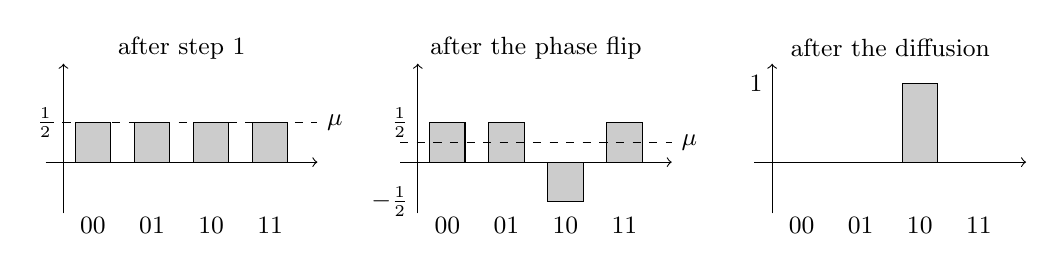
\begin{tikzpicture}[every node/.style={font=\small}, xscale=0.75, yscale=0.5]
        % panel 1
        \begin{scope}
            \draw[->] (-0.3,0) -- (4.3,0);
            \draw[->] (0,-1.3) -- (0,2.5);
            \foreach \x in {0.5,1.5,2.5,3.5} {\draw[fill=gray!40] (\x-0.3,0) rectangle (\x+0.3,1);}
            \foreach \x/\lab in {0.5/00, 1.5/01, 2.5/10, 3.5/11} {\node at (\x,-1.6) {$\lab$};}
            \draw[dashed] (-0.3,1) -- (4.3,1) node[right] {$\mu$};
            \node[left] at (0,1) {$\frac{1}{2}$};
            \node at (2,2.9) {after step 1};
        \end{scope}
        % panel 2
        \begin{scope}[xshift=6cm]
            \draw[->] (-0.3,0) -- (4.3,0);
            \draw[->] (0,-1.3) -- (0,2.5);
            \foreach \x in {0.5,1.5,3.5} {\draw[fill=gray!40] (\x-0.3,0) rectangle (\x+0.3,1);}
            \draw[fill=gray!40] (2.2,0) rectangle (2.8,-1);
            \foreach \x/\lab in {0.5/00, 1.5/01, 2.5/10, 3.5/11} {\node at (\x,-1.6) {$\lab$};}
            \draw[dashed] (-0.3,0.5) -- (4.3,0.5) node[right] {$\mu$};
            \node[left] at (0,1) {$\frac{1}{2}$};
            \node[left] at (0,-1) {$-\frac{1}{2}$};
            \node at (2,2.9) {after the phase flip};
        \end{scope}
        % panel 3
        \begin{scope}[xshift=12cm]
            \draw[->] (-0.3,0) -- (4.3,0);
            \draw[->] (0,-1.3) -- (0,2.5);
            \draw[fill=gray!40] (2.2,0) rectangle (2.8,2);
            \foreach \x/\lab in {0.5/00, 1.5/01, 2.5/10, 3.5/11} {\node at (\x,-1.6) {$\lab$};}
            \node[left] at (0,2) {$1$};
            \node at (2,2.9) {after the diffusion};
        \end{scope}
    \end{tikzpicture}
    \caption{The amplitudes for $N = 4$ and $x^* = 10$ after the Hadamard gates, after the phase flip,
        and after the inversion about the mean $\mu$.}
    \label{fig:grover4-1006}
\end{figure}

\FloatBarrier
\section{Grover's Algorithm on \texorpdfstring{$n$}{n} Qubits}

% Commented out: longer wording of the text that follows.
% For $n$ qubits and a unique solution $x^*$ the same steps apply to the $N$ amplitudes. After the
% Hadamard gates every amplitude is $\sfrac{1}{\sqrt{N}}$. The phase flip makes the amplitude of
% $x^*$ equal to $-\sfrac{1}{\sqrt{N}}$. So the mean is
% $\mu = \sfrac{(N-2)}{(N\sqrt{N})} \approx \sfrac{1}{\sqrt{N}}$ and the diffusion operator maps the
% amplitude of $x^*$ to $2\mu + \sfrac{1}{\sqrt{N}} \approx \sfrac{3}{\sqrt{N}}$. As long as this
% amplitude is small, the mean stays close to $\sfrac{1}{\sqrt{N}}$ and each iteration adds about
% $\sfrac{2}{\sqrt{N}}$ to it. So after about $\sqrt{N}$ iterations it is a constant and a measurement
% finds $x^*$ with constant probability.
For $n$ qubits and a unique solution $x^*$ the same steps apply to the $N$ amplitudes. The Hadamard
gates make every amplitude $\sfrac{1}{\sqrt{N}}$, and the phase flip makes the amplitude of $x^*$
equal to $-\sfrac{1}{\sqrt{N}}$. The mean, and the amplitude of $x^*$ after the diffusion, are
\[\mu = \frac{N-2}{N\sqrt{N}} \approx \frac{1}{\sqrt{N}}, \qquad
    2\mu + \frac{1}{\sqrt{N}} \approx \frac{3}{\sqrt{N}}.\]
While this amplitude is small, the mean stays close to $\sfrac{1}{\sqrt{N}}$ and each iteration adds
about $\sfrac{2}{\sqrt{N}}$ to the amplitude. After about $\sqrt{N}$ iterations it is a constant, and
a measurement finds $x^*$ with constant probability.

\subsection{The Operators \texorpdfstring{$Z_f$}{Zf}, \texorpdfstring{$Z_0$}{Z0} and \texorpdfstring{$D$}{D}}

\paragraph{The phase flip $Z_f$.} The phase flip
\[Z_f \colon \ket{x} \longmapsto (-1)^{f(x)} \ket{x}\]
is implemented by one query $U_f$ with an extra qubit in $H\ket{1} = \frac{1}{\sqrt{2}}(\ket{0} - \ket{1})$
(\cref{fig:zf-1006}). The query leaves the extra qubit unchanged, and a second Hadamard gate returns
it to $\ket{1}$.

\begin{figure}[ht]
    \centering
    \begin{tikzpicture}[scale=0.82, gate/.style={draw, fill=white, minimum size=6mm, inner sep=1pt}]
        \foreach \y in {3,2.25,1} {\draw (0,\y) -- (6,\y);}
        \node at (0.6,1.7) {$\vdots$};
        \node at (5.4,1.7) {$\vdots$};
        \draw (0,-0.25) -- (6,-0.25);
        \node[left] at (0,-0.25) {$\ket{1}$};
        \draw[fill=white] (2.4,-0.7) rectangle (3.6,3.45);
        \node at (3,1.4) {$U_f$};
        \node[gate] at (1.2,-0.25) {$H$};
        \node[gate] at (4.8,-0.25) {$H$};
        \draw[decorate, decoration={brace, amplitude=5pt}] (-0.3,0.8) -- (-0.3,3.2)
        node[midway, left=6pt] {$\ket{x}$};
        \draw[decorate, decoration={brace, amplitude=5pt, mirror}] (6.3,0.8) -- (6.3,3.2)
        node[midway, right=6pt] {$(-1)^{f(x)} \ket{x}$};
        \node[right] at (6.3,-0.25) {$\ket{1}$};
    \end{tikzpicture}
    \caption{The phase flip $Z_f$, implemented with one query $U_f$.}
    \label{fig:zf-1006}
\end{figure}

\paragraph{The phase flip $Z_0$ about $0^n$.} Let $f_0 \colon \set{0,1}^n \to \set{0,1}$ be the function
with $f_0(x) = \bar{x}_1 \wedge \bar{x}_2 \wedge \dots \wedge \bar{x}_n$, where $\bar{x}_i = \neg x_i$,
so $f_0(x) = 1$ only for $x = 0^n$. Its phase flip is
\[Z_0 \colon \ket{x} \longmapsto \begin{cases} -\ket{x} & \text{if } x = 0^n, \\ \ket{x} & \text{otherwise}, \end{cases}
    \qquad \text{so} \qquad Z_0 = I - 2 \ket{0^n}\bra{0^n}.\]
% Commented out: not in the lecture notes.
% As a matrix, $Z_0$ is the $N \times N$ diagonal matrix with $-1$ in the top left corner and $1$
% elsewhere. It is implemented like $Z_f$, with an extra qubit in $H\ket{1}$ and the reversible gate
% $\ket{x}\ket{c} \mapsto \ket{x}\ket{c \oplus (\bar{x}_1 \wedge \dots \wedge \bar{x}_n)}$
% (a Toffoli gate with $n$ negated controls) in place of the black box. It makes no query to $f$.
As a matrix, $Z_0$ is the $N \times N$ diagonal matrix with $-1$ in the top left corner and $1$
elsewhere.

\paragraph{The diffusion operator $D$.} Let $\ket{h} = H^{\otimes n}\ket{0^n} = \frac{1}{\sqrt{N}} \sum_{x} \ket{x}$
be the uniform superposition. The diffusion operator is
\[D = -H^{\otimes n} Z_0 H^{\otimes n}.\]

\begin{lemma}[Inversion About the Mean]\label{lem:diffusion-1006}
    $D = 2\ket{h}\bra{h} - I$, and for every state $\sum_{x} a_x \ket{x}$ with mean amplitude
    $\mu = \frac{1}{N} \sum_{x} a_x$,
    \[D \sum_{x \in \set{0,1}^n} a_x \ket{x} = \sum_{x \in \set{0,1}^n} (2\mu - a_x) \ket{x}.\]
\end{lemma}

\begin{proof}
    Since $H^\dagger = H$ and $H^2 = I$, we have $H^{\otimes n} H^{\otimes n} = I$ and
    $\bra{0^n} H^{\otimes n} = \left(H^{\otimes n}\ket{0^n}\right)^\dagger = \bra{h}$, so
    \[D = -H^{\otimes n} \left(I - 2\ket{0^n}\bra{0^n}\right) H^{\otimes n}
        = -\left(I - 2\ket{h}\bra{h}\right) = 2\ket{h}\bra{h} - I.\]
    For $\ket{\psi} = \sum_x a_x \ket{x}$ we have $\braket{h}{\psi} = \frac{1}{\sqrt{N}} \sum_x a_x = \sqrt{N}\mu$, so
    \[D\ket{\psi} = 2\sqrt{N}\mu \ket{h} - \ket{\psi} = 2\mu \sum_{x} \ket{x} - \sum_{x} a_x \ket{x} = \sum_{x} (2\mu - a_x) \ket{x}. \qedhere\]
\end{proof}

% Commented out: not in the lecture notes.
% So $D$ is the inversion about the mean of step~3, and it makes no query.
So $D$ is the inversion about the mean of step~3.

\paragraph{The Grover iteration.} One iteration of steps 2 and 3 is the operator
\[G = D Z_f = -H^{\otimes n} Z_0 H^{\otimes n} Z_f.\]
Grover's algorithm prepares $\ket{h} = H^{\otimes n}\ket{0^n}$, applies $G$ $k$ times and measures
% Commented out: not in the lecture notes.
% (\cref{fig:grover-circuit-1006}). It makes $k$ queries, one per iteration.
(\cref{fig:grover-circuit-1006}).

\begin{figure}[ht]
    \centering
    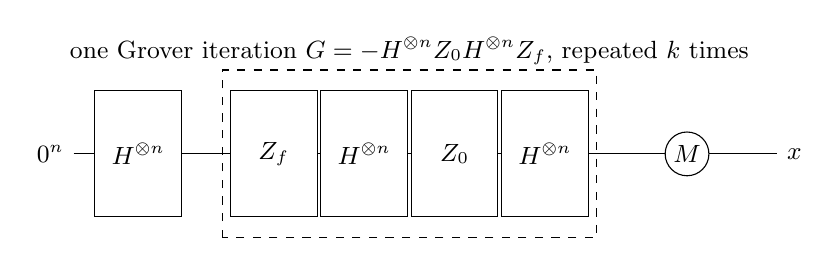
\begin{tikzpicture}[scale=0.82, box/.style={draw, fill=white, minimum height=1.6cm, minimum width=1.1cm, inner sep=2pt},
            meter/.style={draw, circle, fill=white, inner sep=1.5pt}, every node/.style={font=\small}]
        \node[left] at (0,0) {$\ket{0^n}$};
        \draw (0,0) -- (10.9,0);
        \node[box] at (1,0) {$H^{\otimes n}$};
        \node[box] at (3.1,0) {$Z_f$};
        \node[box] at (4.5,0) {$H^{\otimes n}$};
        \node[box] at (5.9,0) {$Z_0$};
        \node[box] at (7.3,0) {$H^{\otimes n}$};
        \node[meter] at (9.5,0) {$M$};
        \draw[dashed] (2.3,-1.3) rectangle (8.1,1.3);
        \node at (5.2,1.6) {one Grover iteration $G = -H^{\otimes n} Z_0 H^{\otimes n} Z_f$, repeated $k$ times};
        \node[right] at (10.9,0) {$x$};
    \end{tikzpicture}
    \caption{Grover's algorithm on $n$ qubits (the extra qubit used by $Z_f$ and $Z_0$ is not drawn).}
    \label{fig:grover-circuit-1006}
\end{figure}

\section{Analysis: A Rotation in Two Dimensions}\label{sec:grover-analysis-1006}

Let $f$ have $a$ solutions, $1 \leq a \leq N - 1$, and let $b = N - a$. Let
\[\ket{A} = \frac{1}{\sqrt{a}} \sum_{\substack{x \in \set{0,1}^n \\ f(x) = 1}} \ket{x},
    \qquad
    \ket{B} = \frac{1}{\sqrt{b}} \sum_{\substack{x \in \set{0,1}^n \\ f(x) = 0}} \ket{x}\]
% Commented out: longer wording of the text that follows.
% be the uniform superpositions of the solutions and of the non-solutions. They are unit vectors, and
% they are orthogonal since no basis state appears in both. The whole computation stays in the plane
% they span. The initial state is
be the uniform superpositions of the solutions and of the non-solutions. They are unit vectors,
orthogonal since no basis state appears in both. The computation stays in their plane. The initial
state is
\begin{equation}\label{eq:h-AB-1006}
    \ket{h} = \frac{1}{\sqrt{N}} \sum_{x \in \set{0,1}^n} \ket{x}
    = \frac{1}{\sqrt{N}} \left(\sqrt{a} \ket{A} + \sqrt{b} \ket{B}\right)
    = \sqrt{\frac{a}{N}} \ket{A} + \sqrt{\frac{b}{N}} \ket{B}.
\end{equation}
Since $\frac{a}{N} + \frac{b}{N} = 1$, there is a unique angle $\theta \in (0, \sfrac{\pi}{2})$ with
\[\sin\theta = \sqrt{\frac{a}{N}}, \qquad \cos\theta = \sqrt{\frac{b}{N}},
    \qquad \text{so that} \qquad \ket{h} = \sin\theta \ket{A} + \cos\theta \ket{B}.\]
For a unique solution, $\sin\theta = \sfrac{1}{\sqrt{N}}$, so $\theta \approx \sfrac{1}{\sqrt{N}}$ and
$\ket{h}$ is almost $\ket{B}$ (\cref{fig:rotation-1006}).

\begin{lemma}[One Grover Iteration]\label{lem:giter-1006}
    \begin{align*}
        G\ket{A} & = \left(1 - \frac{2a}{N}\right)\ket{A} - \frac{2\sqrt{ab}}{N}\ket{B}
        = \cos 2\theta \ket{A} - \sin 2\theta \ket{B},                                 \\
        G\ket{B} & = \frac{2\sqrt{ab}}{N}\ket{A} - \left(1 - \frac{2b}{N}\right)\ket{B}
        = \sin 2\theta \ket{A} + \cos 2\theta \ket{B}.
    \end{align*}
\end{lemma}

\begin{proof}
    % Commented out: longer wording of the text that follows.
    % By the definition of $Z_f$, $Z_f\ket{A} = -\ket{A}$ and $Z_f\ket{B} = \ket{B}$. By
    % \cref{eq:h-AB-1006} and orthonormality, $\braket{h}{A} = \sqrt{a/N}$ and
    % $\braket{h}{B} = \sqrt{b/N}$. With $D = 2\ket{h}\bra{h} - I$ (\cref{lem:diffusion-1006}),
    % substituting \cref{eq:h-AB-1006} for $\ket{h}$ in the last step of each line,
    We have $Z_f\ket{A} = -\ket{A}$ and $Z_f\ket{B} = \ket{B}$. By \cref{eq:h-AB-1006} and
    orthonormality, $\braket{h}{A} = \sqrt{a/N}$ and $\braket{h}{B} = \sqrt{b/N}$. With
    $D = 2\ket{h}\bra{h} - I$ (\cref{lem:diffusion-1006}) and \cref{eq:h-AB-1006} in the last step,
    \begin{align*}
        G\ket{A} = -D\ket{A} & = \ket{A} - 2\ket{h}\braket{h}{A} = \ket{A} - 2\sqrt{\frac{a}{N}} \ket{h}
        = \left(1 - \frac{2a}{N}\right)\ket{A} - \frac{2\sqrt{ab}}{N}\ket{B}, \\
        G\ket{B} = D\ket{B}  & = 2\ket{h}\braket{h}{B} - \ket{B} = 2\sqrt{\frac{b}{N}} \ket{h} - \ket{B}
        = \frac{2\sqrt{ab}}{N}\ket{A} - \left(1 - \frac{2b}{N}\right)\ket{B}.
    \end{align*}
    % Commented out: longer wording of the text that follows.
    % The trigonometric form follows from $\sin^2\theta = \sfrac{a}{N}$, $\cos^2\theta = \sfrac{b}{N}$ and
    % the double angle formulas: $\cos 2\theta = 1 - 2\sin^2\theta = 1 - \sfrac{2a}{N}$,
    % $\cos 2\theta = 2\cos^2\theta - 1 = -\left(1 - \sfrac{2b}{N}\right)$ and
    % $\sin 2\theta = 2\sin\theta\cos\theta = \sfrac{2\sqrt{ab}}{N}$.
    The trigonometric form follows from $\sin^2\theta = \sfrac{a}{N}$, $\cos^2\theta = \sfrac{b}{N}$ and
    the double angle formulas:
    \begin{align*}
        \cos 2\theta & = 1 - 2\sin^2\theta = 1 - \frac{2a}{N},                 \\
        \cos 2\theta & = 2\cos^2\theta - 1 = -\left(1 - \frac{2b}{N}\right), \\
        \sin 2\theta & = 2\sin\theta\cos\theta = \frac{2\sqrt{ab}}{N}. \qedhere
    \end{align*}
\end{proof}

% Commented out: longer wording of the text that follows.
% Since $a + b = N$, both $1 - \sfrac{2a}{N}$ and $\sfrac{2b}{N} - 1$ equal $\sfrac{(b - a)}{N}$. We write a
% state $\beta\ket{B} + \alpha\ket{A}$ of the plane as the column vector $(\beta, \alpha)^{T}$ in the basis
% $(\ket{B}, \ket{A})$. Then $G$ acts as the $2 \times 2$ matrix
Since $a + b = N$, both $1 - \sfrac{2a}{N}$ and $\sfrac{2b}{N} - 1$ equal $\sfrac{(b - a)}{N}$. Write
$\beta\ket{B} + \alpha\ket{A}$ as the column vector $(\beta, \alpha)^{T}$ in the basis
$(\ket{B}, \ket{A})$. Then $G$ acts as the matrix
\begin{equation}\label{eq:gmatrix-1006}
    G = \begin{pmatrix} \dfrac{b - a}{N} & -\dfrac{2\sqrt{ab}}{N} \\[2ex] \dfrac{2\sqrt{ab}}{N} & \dfrac{b - a}{N} \end{pmatrix}
    = \begin{pmatrix} \cos 2\theta & -\sin 2\theta \\ \sin 2\theta & \cos 2\theta \end{pmatrix},
\end{equation}
% Commented out: longer wording of the text that follows.
% whose columns are the coordinates of $G\ket{B}$ and $G\ket{A}$. This is the rotation matrix
% $R_{\phi} = \left(\begin{smallmatrix} \cos\phi & -\sin\phi \\ \sin\phi & \cos\phi \end{smallmatrix}\right)$
% with $\phi = 2\theta$. So one Grover iteration \emph{rotates} the plane by the angle $2\theta$, from
% $\ket{B}$ towards $\ket{A}$.
whose columns are the coordinates of $G\ket{B}$ and $G\ket{A}$. This is the rotation matrix
$R_{\phi} = \left(\begin{smallmatrix} \cos\phi & -\sin\phi \\ \sin\phi & \cos\phi \end{smallmatrix}\right)$
with $\phi = 2\theta$: one Grover iteration \emph{rotates} the plane by $2\theta$, from $\ket{B}$
towards $\ket{A}$.

\begin{exercisebox}
\begin{exercise}\label{ex:grover-rotation-1006}
    Compute $G\ket{h} = \sqrt{\sfrac{a}{N}}\, G\ket{A} + \sqrt{\sfrac{b}{N}}\, G\ket{B}$ and
    $G^k\ket{h}$ for $k \geq 0$, and verify that the matrix of $G$ in \cref{eq:gmatrix-1006} is the
    rotation $R_{2\theta}$.
\end{exercise}
\tcblower
\begin{wsolution}
    % Commented out: longer wording of the text that follows.
    % \emph{The matrix is a rotation.} By \cref{lem:giter-1006} and $\sfrac{(b-a)}{N} = 1 - \sfrac{2a}{N} = \sfrac{2b}{N} - 1$,
    % the two columns of the matrix in \cref{eq:gmatrix-1006} are the coordinates of
    % $G\ket{B} = \cos 2\theta \ket{B} + \sin 2\theta \ket{A}$ and $G\ket{A} = -\sin 2\theta \ket{B} + \cos 2\theta \ket{A}$,
    % which are the columns of $R_{2\theta}$ (not $R_\theta$).
    \emph{The matrix is a rotation.} By \cref{lem:giter-1006} and
    $\sfrac{(b-a)}{N} = 1 - \sfrac{2a}{N} = \sfrac{2b}{N} - 1$, the columns of the matrix in
    \cref{eq:gmatrix-1006} are the coordinates of
    \[G\ket{B} = \cos 2\theta \ket{B} + \sin 2\theta \ket{A}, \qquad
        G\ket{A} = -\sin 2\theta \ket{B} + \cos 2\theta \ket{A}.\]
    These are the columns of $R_{2\theta}$ (not $R_\theta$).

    \emph{The state $G\ket{h}$.} By \cref{eq:h-AB-1006}, $\ket{h} = \sin\theta \ket{A} + \cos\theta \ket{B}$.
    By \cref{lem:giter-1006} and the addition formulas for $\sin(\theta + 2\theta)$ and
    $\cos(\theta + 2\theta)$,
    \begin{align*}
        G\ket{h}
         & = \sin\theta \left(\cos 2\theta \ket{A} - \sin 2\theta \ket{B}\right) + \cos\theta \left(\sin 2\theta \ket{A} + \cos 2\theta \ket{B}\right) \\
         & = \sin 3\theta \ket{A} + \cos 3\theta \ket{B}.
    \end{align*}
    With $\sin 3\theta = 3\sin\theta - 4\sin^3\theta$, $\cos 3\theta = 4\cos^3\theta - 3\cos\theta$ and
    $\sfrac{4b}{N} - 3 = 1 - \sfrac{4a}{N}$, this is
    \[G\ket{h} = \sqrt{\frac{a}{N}}\left(3 - \frac{4a}{N}\right)\ket{A} + \sqrt{\frac{b}{N}}\left(1 - \frac{4a}{N}\right)\ket{B}.\]
    The state starts at the angle $\theta$ from $\ket{B}$ and the iteration adds $2\theta$
    (\cref{fig:rotation-1006}).

    % Commented out: longer wording of the text that follows.
    % \emph{The state $G^k\ket{h}$.} The same computation with any angle $\beta$ in place of $\theta$ gives
    % $G\left(\sin\beta \ket{A} + \cos\beta \ket{B}\right) = \sin(\beta + 2\theta) \ket{A} + \cos(\beta + 2\theta) \ket{B}$.
    % So by induction on $k$, starting from the angle $\theta$ of $\ket{h}$,
    \emph{The state $G^k\ket{h}$.} The same computation with any angle $\beta$ in place of $\theta$ gives
    \[G\left(\sin\beta \ket{A} + \cos\beta \ket{B}\right) = \sin(\beta + 2\theta) \ket{A} + \cos(\beta + 2\theta) \ket{B}.\]
    By induction on $k$, starting from the angle $\theta$ of $\ket{h}$,
    \[G^k\ket{h} = \sin\left((2k+1)\theta\right) \ket{A} + \cos\left((2k+1)\theta\right) \ket{B}.\]
\end{wsolution}
\end{exercisebox}

\begin{figure}[ht]
    \centering
    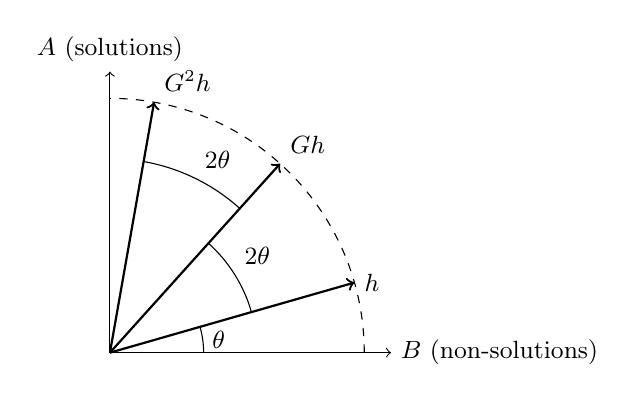
\begin{tikzpicture}[scale=0.85, every node/.style={font=\small}]
        \draw[->] (0,0) -- (4.2,0) node[right] {$\ket{B}$ (non-solutions)};
        \draw[->] (0,0) -- (0,4.2) node[above] {$\ket{A}$ (solutions)};
        \draw[->, thick] (0,0) -- (16:3.8) node[right] {$\ket{h}$};
        \draw[->, thick] (0,0) -- (48:3.8) node[above right] {$G\ket{h}$};
        \draw[->, thick] (0,0) -- (80:3.8) node[above right] {$G^2\ket{h}$};
        \draw (1.4,0) arc (0:16:1.4) node[midway, right] {$\theta$};
        \draw (16:2.2) arc (16:48:2.2) node[midway, above right] {$2\theta$};
        \draw (48:2.9) arc (48:80:2.9) node[midway, above right] {$2\theta$};
        \draw[dashed] (3.8,0) arc (0:90:3.8);
    \end{tikzpicture}
    \caption{Grover's algorithm in the plane spanned by $\ket{A}$ and $\ket{B}$ for
        $\theta = 16^\circ$.}
    \label{fig:rotation-1006}
\end{figure}

The number of iterations is computed in the next lecture (\cref{sec:iterations-1008}).

\FloatBarrier
